\documentclass[00-GLMregslides.tex]{subfiles}
\begin{document}
%================================================ %
%\begin{frame}[fragile]
%	\frametitle{Ordered logistic regression \texttt{R} }
%	\Large
%%s[, 4] <- s[, 4] - s[, 3]
%%s[, 3] <- s[, 3] - s[, 3]
%%s # print
%%## as.numeric(apply)    N=400
%%## 
%%## +-------+-----------+---+----+----+------+
%%## |       |           |N  |Y>=1|Y>=2|Y>=3  |
%%## +-------+-----------+---+----+----+------+
%%## |pared  |No         |337|Inf |0   |-2.062|
%%## |       |Yes        | 63|Inf |0   |-2.113|
%%## +-------+-----------+---+----+----+------+
%%## |public |No         |343|Inf |0   |-2.140|
%%## |       |Yes        | 57|Inf |0   |-1.372|
%%## +-------+-----------+---+----+----+------+
%%## |gpa    |[1.90,2.73)|102|Inf |0   |-2.375|
%%## |       |[2.73,3.00)| 99|Inf |0   |-2.038|
%%## |       |[3.00,3.28)|100|Inf |0   |-1.890|
%%## |       |[3.28,4.00]| 99|Inf |0   |-1.864|
%%## +-------+-----------+---+----+----+------+
%%## |Overall|           |400|Inf |0   |-1.997|
%%## +-------+-----------+---+----+----+------+
%\end{frame}

%================================================ %
\begin{frame}[fragile]
	\frametitle{Ordered logistic regression \texttt{R} }
	\Large
\begin{framed}
\begin{verbatim}
plot(s, which=1:3, pch=1:3, 
    xlab='logit', main=' ', 
    xlim=range(s[,3:4]))
\end{verbatim}
\end{framed}
\end{frame}

%================================================ %
\begin{frame}[fragile]
	\frametitle{Ordered logistic regression \texttt{R} }
	\Large
	
%Plot viewing proportional odds assumption

\begin{itemize}
\item Once we are done assessing whether the assumptions of our model hold, we can obtain predicted probabilities, which are usually easier to understand than either the coefficients or the odds ratios. 

\item For example, we can vary gpa for each level of pared and public and calculate the probability of being in each category of apply. 
\item We do this by creating a new dataset of all the values to use for prediction.
\end{itemize}
\end{frame}

%================================================ %
\begin{frame}[fragile]
\frametitle{Ordered logistic regression \texttt{R} }
\Large
\begin{framed}
\begin{verbatim}
newdat <- data.frame(
  pared = rep(0:1, 200),
  public = rep(0:1, each = 200),
  gpa = rep(seq(from = 1.9, to = 4, 
      length.out = 100), 4))

newdat <- cbind(newdat, predict(m, 
   newdat, type = "probs"))

\end{verbatim}
\end{framed}

\end{frame}

%================================================ %
\begin{frame}[fragile]
	\frametitle{Ordered logistic regression \texttt{R} }
\normalsize

\begin{verbatim}
# Show first few rows
head(newdat)
  pared public   gpa unlikely somewhat likely very likely
1     0      0 1.900   0.7376          0.2205     0.04192
2     1      0 1.921   0.4932          0.3946     0.11221
3     0      0 1.942   0.7325          0.2245     0.04299
4     1      0 1.964   0.4867          0.3985     0.11484
5     0      0 1.985   0.7274          0.2285     0.04407
6     1      0 2.006   0.4802          0.4023     0.11753
\end{verbatim}


\end{frame}

%================================================ %
\begin{frame}[fragile]
	\frametitle{Ordered logistic regression \texttt{R} }
	\Large
	\begin{itemize}
\item Now we can reshape the data long with the reshape2 package and plot all of the predicted probabilities for the different conditions. 
\item We plot the predicted probilities, connected with a line, coloured by level of the outcome, apply, and facetted by level of pared and public.
\item We also use a custom label function, to add clearer labels showing what each column and row of the plot represent.
\end{itemize}
\end{frame}

%================================================ %
\begin{frame}[fragile]
	\frametitle{Ordered logistic regression \texttt{R} }
\normalsize
\large
\begin{framed}
	\begin{verbatim}
	library(reshape2)
	
lnewdat <- melt(newdat, 
  id.vars = c("pared", "public", "gpa"),
  variable.name = "Level", 
  value.name="Probability")
\end{verbatim}
\end{framed}
\end{frame}
%================================================ %
\begin{frame}[fragile]
	\frametitle{Ordered logistic regression \texttt{R} }
	\large
	\begin{framed}
		\begin{verbatim}
%## view first few rows
%head(lnewdat)
%##   pared public   gpa    Level Probability
%## 1     0      0 1.900 unlikely      0.7376
%## 2     1      0 1.921 unlikely      0.4932
%## 3     0      0 1.942 unlikely      0.7325
%## 4     1      0 1.964 unlikely      0.4867
%## 5     0      0 1.985 unlikely      0.7274
%## 6     1      0 2.006 unlikely      0.4802
\end{verbatim}
\end{framed}
\end{frame}
%================================================ %
\begin{frame}[fragile]
	\frametitle{Ordered logistic regression \texttt{R} }
\large
\begin{framed}
\begin{verbatim}
ggplot(lnewdat, aes(x = gpa, y = Probability, 
  colour = Level)) +
  geom_line() +
  facet_grid(pared ~ public, scales="free",
    labeller=function(x, y) sprintf("%s = %d", x, y))
    
\end{verbatim}
\end{framed}

\end{frame}

\begin{frame}
	
	
\begin{figure}
\centering
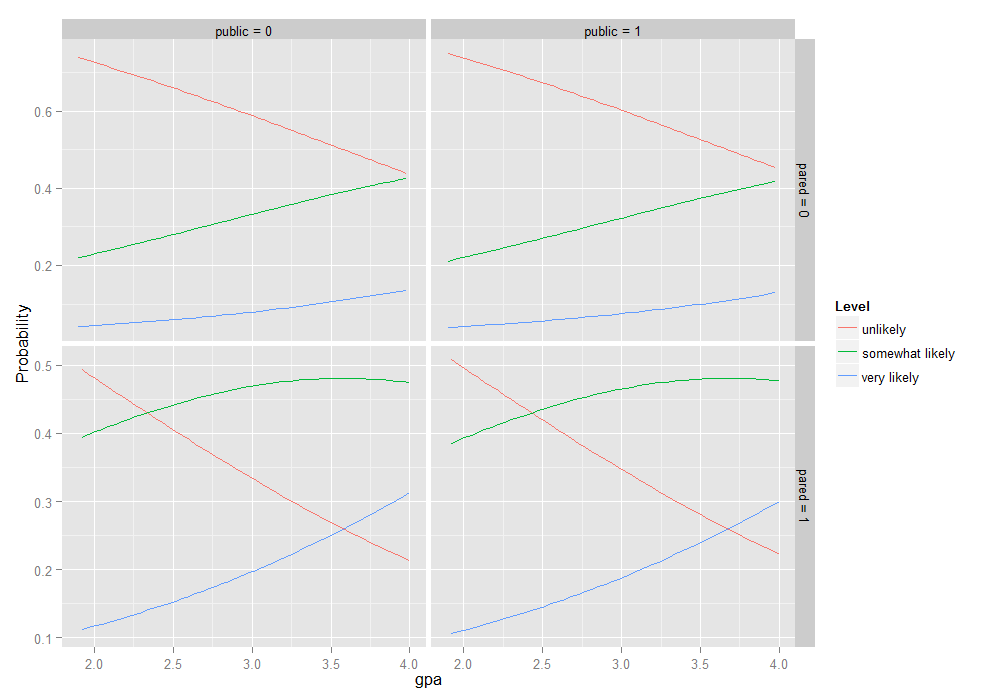
\includegraphics[width=0.99\linewidth]{ologit3}
%\caption{}
%\label{fig:ologit3}
\end{figure}
	
\end{frame}
%================================================ %
\begin{frame}[fragile]
	\frametitle{Ordered logistic regression \texttt{R} }
	\Large
%Plot of predicted probabilities for each group
\textbf{Things to consider
}
\textbf{Perfect prediction: }Perfect prediction means that one value of a predictor variable is associated with only one value of the response variable. 
%If this happens, Stata will usually issue a note at the top of the output and will drop the cases so that the model can run.
\end{frame}

%================================================ %
\begin{frame}[fragile]
	\frametitle{Ordered logistic regression \texttt{R} }
	\Large
\textbf{Sample size:} Both ordered logistic and ordered probit, using maximum likelihood estimates, require sufficient sample size.
% How big is big is a topic of some debate, but they almost always require more cases than OLS regression.
\\
\textbf{Empty cells or small cells:} You should check for empty or small cells by doing a crosstab between categorical predictors and the outcome variable. If a cell has very few cases, the model may become unstable or it might not run at all.
\end{frame}

%================================================ %
\begin{frame}[fragile]
	\frametitle{Ordered logistic regression \texttt{R} }
	\Large
\textbf{Pseudo-R-squared: }There is no exact analog of the R-squared found in OLS. There are many versions of pseudo-R-squares. Please see Long and Freese 2005 for more details and explanations of various pseudo-R-squares.



\textbf{Diagnostics:} Doing diagnostics for non-linear models is difficult, and ordered logit/probit models are even more difficult than binary models.
\end{frame}


%================================================== %	
\end{document}
